We evaluated four regularized estimators denoted here as A, B, C, and D.  Their target estimates correspond to covariance matrices of Gaussian graphical models depicted in Figure 2 where green spheres represent the recorded neurons,  light-colored spheres represent latent units of the graphical model, and edges connecting them represent conditional dependencies or interactions.

\begin{figure}[htp]
\centering
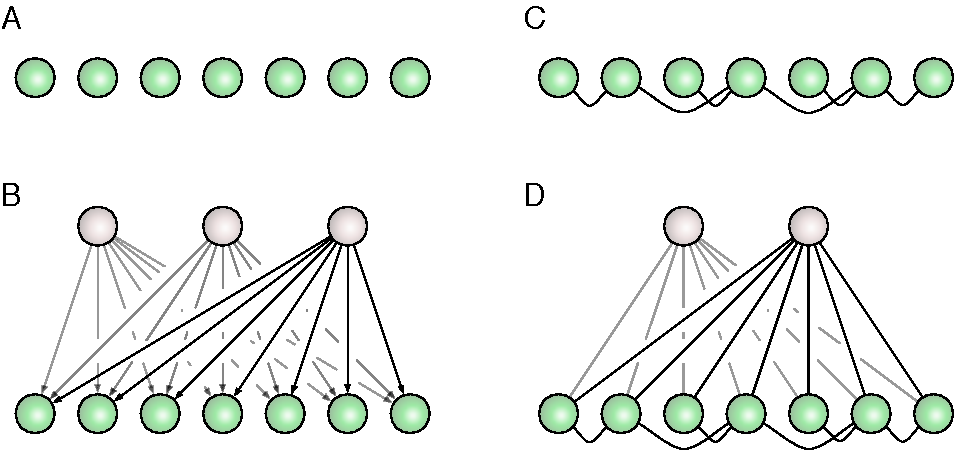
\includegraphics[width=0.5\textwidth]{figures/Figure2.pdf}
\caption{
Graphical models corresponding to the low-dimensional targets of the four regularization schemes used in the paper.
\textbf{A}: A diagonal matrix corresponds to a Gaussian graphical model with no dependencies.
\textbf{B}: In factor analysis, observed nodes are assumed to be influenced by several latent units (``factors") but are otherwise independent.
\textbf{C}: Graphical model with conditional dependencies between a specified subset of pairs of observed neurons, no latent units. 
\textbf{D}: Graphical model with conditional dependencies between a specified subset of pairs of observed neurons and dense interactions with a few latent units.
}\label{fig:02}
\end{figure}


A \emph{graphical model} is a multivarate probability distribution with a specified graph of conditional dependencies between its variables \cite{Koller:2009}.  When this distribution is a multivariate normal distribution, the model becomes a \emph{Gaussian graphical model} (GGM) or, equivalently, a \emph{Gaussian Markov Random Field}.  Gaussian graphical models have a straightforward relationship to their covariance matrix $\Sigma$:  Zero elements in the inverse of $\Sigma$ indicate conditional independence between the corresponding pair of variables.  

Fitting a graphical model to data involves two tasks: (1) the selection of the set of non-zero covariances or \emph{covariance selection} \cite{Dempster:1972} and (b) the fitting of the non-zero elements.

\subsubsection*{Estimator $\mathcal A$: Shrinkage toward diagonal.}
\emph{Estimator $\mathcal A$} shrinks the sample covariance matrix $\hat\Sigma_0$ toward an independent model of the type show in Fig.~\ref{fig:02}A.  The covariance matrix of a GGM in which all units are independent will be diagonal.  
For example, we  could leave the sample variances on the diagonal and zero out the off-diagonal products, making the target estimate 
\begin{equation}\label{eq:sampleVariance}
\hat T= \hat\Sigma_0\circ I
\end{equation}
where $\circ$ denotes the entrywise matrix product (Hadamard product). 
Alternatively, the target could have equal variances, all equal to the average sample variance in the population $v = \frac 1 p \Tr(\hat\Sigma_0)$.
\begin{equation}\label{eq:equalVariance}
\hat T=\frac 1 p \Tr(\hat\Sigma_0) I
\end{equation}
The equal-variance target in Eq.~\ref{eq:equalVariance} has only one degree of freedom and thus lower estimation error but higher bias than the target with sample variances in Eq.~\ref{eq:sampleVariance}. It is not immediately clear which target is better in a particular application. We therefore use the linear mixture of the two targets paramaterized by the mixing coefficient $\alpha\in[0,1]$:
\begin{equation}
\hat T_\alpha = (1-\alpha)(\hat\Sigma_0 \circ I) + \frac \alpha p \mbox{tr}(\hat \Sigma_0)I
\end{equation}
Then the estimator $\hat\Sigma_{\alpha,\lambda}$ is the linear shrinkage of the sample covariance matrix $\hat\Sigma_0$ toward $\hat T_\alpha$ controlled by the mixing proportion $\lambda\in[0,1]$:
\begin{equation}
\hat\Sigma_{\alpha,\lambda}^\mathcal{A} = (1-\lambda)\hat\Sigma_0 + \lambda\hat T_\alpha 
\end{equation}
This covariance matrix estimator is implemented by R's {\tt corpcor} package \cite{Schaefer:2010} and enjoys widespread use in many applications \cite{Schafer:2005}.

We estimated the optimal values of hyperparameters $ \alpha$ and $ \lambda$  by  cross-validation within the training dataset. \TODO{more detail?} \TODO{discuss analytic optimization of shrinkage intensities.}

\subsubsection*{Estimate $\mathcal B$: Shrinkage toward a factor model}
\emph{Estimator $\mathcal B$} shrinks the sample covariance matrix $\hat\Sigma_0$ toward a target estimated by \emph{factor analysis} with $d$ factors, which corresponds to graphical models of the kind in Fig.~\ref{fig:02}B. For multivariate normal distributions, factor analysis estimates a graphical model in which the observed units do not interact directly but are influenced by $d$ common inputs.

The target estimate is then 
\begin{equation}
\hat T_d = \hat L_d + \hat \Psi
\end{equation}
where $\hat L_d$ is a $p\times p$ matrix of rank $d$ and $\hat \Psi$ is a $p\times p$ diagonal matrix. The value of $\hat T_d$ is found by minimizing $\loss{\hat T_d, \hat\Sigma_0}$.

Just as in estimator $\mathcal A$, $\hat\Sigma_0$ is shrunk toward $\hat T_d$ by linear mixing controlled by shrinkage intensity $\lambda\in[0,1]$.
\begin{equation}
\hat\Sigma_{d,\lambda}^\mathcal{B} = (1-\lambda)\hat\Sigma_0 + \lambda\hat T_d
\end{equation}
and the optimal values of $d$ and $\lambda$ are found by cross-validation within the training set.

Factor analysis has a rich history of testing hypotheses about the dominance of a few common inputs \cite{findagoodone}.  In neuroscience, the hypothesis that the population activity in small local circuits is largely driven by a few latent factors has been investigated \cite{Yu:2009,Ecker:2013}.  Estimation of covariance matrices by shrinkage toward a factor model has been used in finance for portfolio risk assessment \cite{Ledoit:2003,Fan:2008}.

\subsubsection*{Estimator $\mathcal C$: Spare inverse}
\emph{Estimator $\mathcal C$} produces a low-dimensional estimate by finding an approximation of $\hat\Sigma_0$ that has many zeros in its inverse. This approximation problem is known as \emph{covariance selection} \cite{Dempster:1972}.  Covariance matrices of this family correspond to graphical models of the type depicted in Fig.~\ref{fig:02}C.

For Gaussian Graphical Models, zeros in the inverse covariance matrix indicate statisitcal independence between the corresponding pairs. Thus the inverse covariance matrix $S=-\Sigma^{-1}$ is also the adjacency matrix of the GGM, indicating which pairs are conditionally dependent. \TODO{discuss how quickly (or slowly) this breaks down with deviations from gaussianity, e.g.~MaxEnt models, Ising models.} \TODO{Also, motivate this from the perpsective of linear regression as in \cite{Varoquaux:2012}.} The off-diagonal elements of $S$ are proportional to partial pairwise correlations between corresponding pairs of neurons. \TODO{Expand.} Regularization of covariance matrix estimation by sparsifying the inverse of the estimate has been using in function genomics \cite{Schafer:2005,other} and fMRI functional connectivity \cite{Varoquaux:2012}. 

The covariance matrix estimate is then 
\begin{equation}
\hat\Sigma_\rho = \hat S^{-1}
\quad\mbox{with}\quad
\hat S = \argmin\limits_{\substack{S\succ 0 \\ \|S\|_0 \le \rho}} \loss{S^{-1},\hat\Sigma_0}   
\end{equation}
where $S\succ 0$ signifies the constraint that $S$ be positive-definite. $\|S\|_0\le\rho$ signifies the constraint  that matrix $S$ have at most $\rho$ non-zero coefficients.
Solving this approximation in this form is computationally challenging. The problem can be made computationally tractable by relaxing \TODO{use "complex relaxation"} the $L_0$ norm to the $L_1$ norm, which converts the problem into one of convex optimization \cite{Donoho:2000}.  The resulting algorithm, known as \emph{graphical lasso} or \emph{GLASSO}  \cite{Meinshausen:2006,Yuan:2007,Banerjee:2008,Friedman:2008}, produces the following estimator  
\begin{equation}
\hat\Sigma_\lambda^\mathcal{C} = \hat S^{-1}
\quad\mbox{with}\quad
\hat S = \argmin\limits_{S\succ 0} \loss{S^{-1},\hat\Sigma_0} + \lambda \|S\|_1
\end{equation}
where $\lambda \|S\|_1$ is the $L_1$ norm of the matrix. \TODO{clarify}.

Just as in the previous estimators, the optimal value of the regularization parameter $\lambda$ is found from training data by cross-validation.

\subsubsection*{Estimator $\mathcal D$: Sparse + low-rank inverse}
\emph{Estimator $\mathcal D$} produces a low-dimensional estimate by approximating $\hat\Sigma_0$ with a matrix whose inverse is the sum of a spase matrix and a low-rank matrix. Covariance matrices of this form correspond to Gaussian graphical models of the form depicted in Fig.~\ref{fig:02}D.

The inverse $S=\Sigma^{-1}$ of the covariance matrix of a GGM constitutes the graph of conditional dependencies (interactions) between the units.  With the assumption of sparse organization of interactions in the network, $S$ is assumed to be sparse.  When the observed units are part of a larger GGM that includes other latent units, let the negative inverse $S^*$ of the joint distribution of both observed and latent units be composed of four partitions
\begin{equation}
S^* = 
\begin{pmatrix}
S_{11} & S_{12} \\
S_{12}^\T & S_{22} 
\end{pmatrix}
\end{equation}
where partition $S_{11}$ describes the interactions between the visible units, $S_{12}$ describe the interactions between visible and latent units, and $S_{22}$ describes the interactions between the latent units. 
Then the covariance matrix of between the observed unit is 
\begin{equation}
\Sigma = \left(S_{11} - S_{12}S_{22}^{-1}S_{12}^\T\right)^{-1}
\end{equation} 
The rank of matrix $S_{12}S_{22}^{-1}S_{12}$ equals the number of latent units. Rather than solving for the precise dependency structure with and between latent units in matrices $S_{12}$ and $S_{22}$, we simply replace the matrix $ S_{12}S_{22}^{-1}S_{12}$ with one low-rank matrix $L= S_{12}S_{22}^{-1}S_{12}$.

Then we obtain estimator $\hat\Sigma_{d,\rho}$, parameterized by the sparsity parameter $\rho$ and  the number of latent units $d$:
\begin{equation}
\hat\Sigma_{d,\rho} = \left(\hat S-\hat L\right)^{-1}
\quad\mbox{where}\quad
(\hat S, \hat L) = \argmin\limits_{\substack{S,L\\ (S-L)\succ 0 \\ \|S\|_0\le\rho \\ L\succeq 0 \\ \rank(L) \le d}} \loss{(S-L)^{-1},\Sigma_0}
\end{equation}

Again, in this formulation, the approximation problem is computationally intractible.  The problem can be made convex by replacing the $L_0$ norm with $L_1$ norm. The resulting algorith, known as \emph{latent-variable graphical lasso} or \emph{LV-GLASSO} \cite{Chandrasekaran:2010,Ma:2013}, produces estimator $\hat\Sigma_{d,\lambda}^{\mathcal D}$:
\begin{equation}
\hat\Sigma_{d,\lambda} ^{\mathcal D} = \left(\hat S-\hat L\right)^{-1}
\quad\mbox{where}\quad
(\hat S, \hat L) = \argmin\limits_{\substack{ S,L \\ (S-L)\succ 0 \\ L\succeq 0 \\ \rank(L) \le d}} \loss{(S-L)^{-1},\Sigma_0} + \lambda \| S \|_1 
\end{equation}
The optimal values of hyperparameters $\lambda$ and $d$ are found cross-validation within the training dataset.
